\documentclass[a4paper, fleqn]{article}
\usepackage{header}
\pgfplotsset{compat=1.17}
\usepgfplotslibrary{fillbetween}
\usetikzlibrary{patterns}

\title{Семинарский лист 2.5}
\author{
    % Александр Богданов   \\ \href{https://t.me/SphericalPotatoInVacuum}{Telegram} \and
    % Алиса Вернигор       \\ \href{https://t.me/allisyonok}{Telegram} \and
    % Анастасия Григорьева \\ \href{https://t.me/weifoll}{Telegram} \and
    % Василий Шныпко       \\ \href{https://t.me/yourvash}{Telegram} \and
    % Данил Казанцев       \\ \href{https://t.me/vserosbuybuy}{Telegram} \and
    Денис Козлов         \\ \href{https://t.me/DKozl50}{Telegram} \and
    Елизавета Орешонок   \\ \href{https://t.me/eaoresh}{Telegram} \and
    Ира Голобородько     \\ \href{https://t.me/Ira4kgl}{Telegram}
    % Иван Пешехонов       \\ \href{https://t.me/JohanDDC}{Telegram} \and
    % Иван Добросовестнов  \\ \href{https://t.me/ivankot13}{Telegram} \and
    % Настя Городилова     \\ \href{https://t.me/nastygorodi}{Telegram} \and
    % Никита Насонков      \\ \href{https://t.me/nnv_nick}{Telegram} \and
    % Сергей Лоптев        \\ \href{https://t.me/beast_sl}{Telegram}
}

\date{Версия от {\ddmmyyyydate\today} \currenttime}

\begin{document}
    \maketitle
    
    \section*{Задайте в полярных координатах множество $D$, заданное неравенствами в декартовых координатах.
    Предполагая функцию $f$ непрерывной на $D$, преобразуйте интеграл в полярных координатах к повторному.}
    % \subsection*{Задача 1}
    
    % \subsection*{Задача 2}
    
    % \subsection*{Задача 3}
    
    % \subsection*{Задача 4}
    
    % \subsection*{Задача 5}
    
    % \subsection*{Задача 6}
    
    \section*{Перейдя к полярным координатам, вычислите интеграл.}
    % \subsection*{Задача 7}
    
    \subsection*{Задача 8}
    \begin{flalign*}
        & \iint\limits_D \frac{x dxdy}{\sqrt{4 - x^2 - y^2}}, \;\; D = \left\{ (x, y) | x^2 + y^2 \leq 2x \right\} \\
        & \begin{cases} 
            x = r \cos \varphi \\
            y = r \sin \varphi 
        \end{cases} \Rightarrow D = \left\{ (r, \varphi) | r \leq 2 \cos \varphi \right\} \\
        & \iint\limits_D \frac{r \cos \varphi}{\sqrt{4 - r^2}} r d \varphi d r = 
        \int\limits_{0}^{2} dr \int\limits_{-\arccos \left( r/2 \right)}^{\arccos \left( r/2 \right)} 
        \frac{r^2 \cos \varphi}{\sqrt{4 - r^2}} d \varphi = 
        \int\limits_{0}^{2} \frac{r^2}{\sqrt{4 - r^2}} dr 
        \int\limits_{-\arccos \left( r/2 \right)}^{\arccos \left( r/2 \right)} 
        \cos \varphi d \varphi = \\
        & = \int\limits_{0}^{2} \frac{r^2}{\sqrt{4 - r^2}} dr 
        \left. \sin \varphi \right|_{-\arccos \left( r/2 \right)}^{\arccos \left( r/2 \right)} = 
        \int\limits_{0}^{2} \frac{r^2}{\sqrt{4 - r^2}} \sqrt{4 - r^2} dr = \int_0^2 r^2 dr = \frac{8}{3}
    \end{flalign*}
    
    \section*{Перейдите к переменным, в которых область интегрирования имеет вид прямоугольника, 
    и вычислите интеграл.}
    % \subsection*{Задача 9}
    
    \subsection*{Задача 10}
    \begin{flalign*}
        & \iint\limits_D xy(x+y) dxdy, \;\;\;\;\;\; D = \left\{ (x, y) \Big| -1 \leq x - y \leq 1, 
        \frac{1}{x} \leq y \leq \frac{2}{x} \right\} \\
        & \begin{cases} 
            u = x - y & u \in [-1, 1]\\
            v = xy & v \in [1, 2]
        \end{cases} \Rightarrow x = u + y \Rightarrow v = uy + y^2 \Rightarrow y = \frac{-u \pm \sqrt{u^2 + 4v}}{2} \\
        & u^2 + 4v \geq 4 \Rightarrow \sqrt{u^2 + 4v} \geq 2 \Rightarrow y_{-} \leq \frac{-u - 2}{2} \Rightarrow y_{-} < 0.
        \text{ По картинке } y > 0 \Rightarrow y = y_{+} = \frac{-u + \sqrt{u^2 + 4v}}{2} \\
        & x = u + y = u + \frac{-u + \sqrt{u^2 + 4v}}{2} = \frac{u + \sqrt{u^2 + 4v}}{2} \\
        & \begin{cases} 
            x = \frac{u + \sqrt{u^2 + 4v}}{2} \\
            y = \frac{-u + \sqrt{u^2 + 4v}}{2}  
        \end{cases} \Rightarrow J = \begin{pmatrix}
            \frac{1}{2} + \frac{u}{2\sqrt{u^2 + 4v}} & \frac{1}{\sqrt{u^2 + 4v}} \\
            - \frac{1}{2} + \frac{u}{2\sqrt{u^2 + 4v}} & \frac{1}{\sqrt{u^2 + 4v}} \\
        \end{pmatrix} \;\;\;\;\;\; |J| = \frac{1}{\sqrt{u^2 + 4v}} \\
        & \int\limits_{-1}^1 du \int\limits_1^2 
        v \left( \frac{u + \sqrt{u^2 + 4v}}{2} + \frac{-u + \sqrt{u^2 + 4v}}{2} \right) |J| dv = 
        \int\limits_{-1}^1 du \int\limits_1^2 v \frac{\sqrt{u^2 + 4v}}{\sqrt{u^2 + 4v}} dv = 
        \int\limits_{-1}^1 du \int\limits_1^2 v dv = 3
    \end{flalign*}

    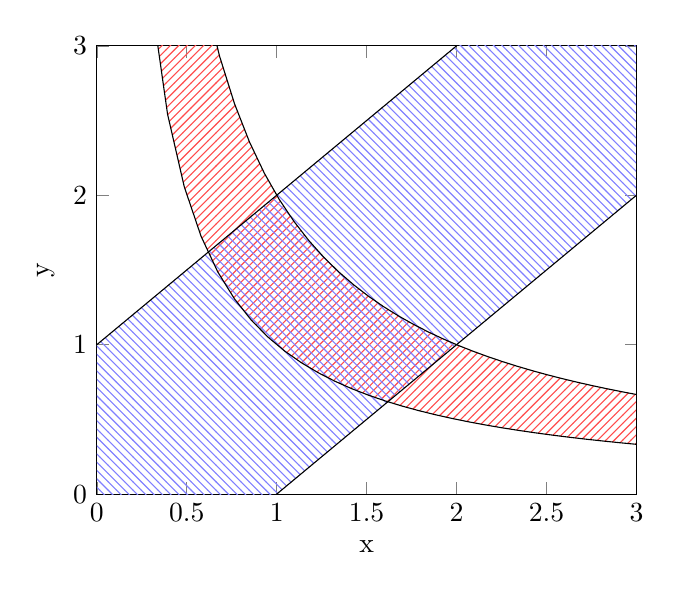
\begin{tikzpicture} 
        \begin{axis}[xmin=0, xmax=3, ymin=0, ymax=3, xlabel=x, ylabel=y]
            \addplot[domain=0.3:3, samples=30, variable=\x, name path=A] ({\x}, {1/\x});
            \addplot[domain=0.6:3, samples=30, variable=\x, name path=B] ({\x}, {2/\x});
            \addplot[pattern color=red!70, pattern=north east lines] fill between [of=A and B];
            \addplot[domain=0:3, name path=C] {x+1};
            \addplot[domain=0:3, name path=D] {x-1};
            \addplot[pattern color=blue!50, pattern=north west lines] fill between [of=C and D];
        \end{axis} 
    \end{tikzpicture}   
    
    % \subsection*{Задача 11}
    
    % \subsection*{Задача 12}
    
    \section*{Задайте в цилиндрических координатах множество $D$, заданное неравенствами в декартовых
    координатах. Пердполагаю функцию $f$ непрерывной на $D$, преобразуйте интеграл в цилиндрических
    координатах к повторному.}
    % \subsection*{Задача 13}
    
    % \subsection*{Задача 14}
    
    \section*{Перейдя к цилиндрическим координатам, вычислите интеграл.}
    \subsection*{Задача 15}
    \begin{flalign*}
        & \iiint\limits_D z dxdydz \;\;\;\;\;\; D = \left\{ (x, y, z) | x^2 + y^2 \leq z^2, \; 0 \leq z \leq 1 \right\} 
        \Rightarrow D = \left\{ (r, \varphi, z) | r^2 \leq z^2, \; 0 \leq z \leq 1 \right\} \\
        & \int_{0}^{2\pi} d\varphi \int_0^1 z  dz \int_0^z r dr = 
        \int_{0}^{2\pi} d\varphi \int_0^1 z \frac{z^2}{2} dz = 
        2 \pi \frac{1}{8} = \frac{\pi}{4} 
    \end{flalign*}
    
    % \subsection*{Задача 16}
    
    \section*{Задайте в сферических координатах множество $D$, заданное неравенствами в декартовых координатах.
    Предполагая функцию $f$ непрерывной на $D$, преобразуйте интеграл в сферических координатах к повторному.}
    % \subsection*{Задача 17}
    
    % \subsection*{Задача 18}
    
    \section*{Перейдя к сферическим координатам, вычислите интеграл.}
    % \subsection*{Задача 19}
    
    % \subsection*{Задача 20}
    
\end{document}
